% (c) Jakub Stejskal
% Master Thesis
% Performance Testing and Analysis of Qpid-Dispatch Router
% Chapter 5
\chapter{Implementation}
\label{Implementation}
This chapter describes the implementation of components, which were described in the Chapter \ref{Analysis and Design}. The main part is the Agent module for MPT, which is implemented in Java and Groovy language. The second part is Topology Generator, which is python package for automatic generation of dispatch topology based on user's metadata. Since topology deployment is not part MPT or Topology Generator, there is also described \emph{Ansible} script for it. Measurement data gathering and reporting is done by MPT parts that has already been mentioned in the Chapter \ref{Analysis and Design}.

\section{Topology Generation}
Qpid-dispatch has a lot of configurable attributes, which can influence router behavior. These attributes can be set up with an AMQP management tool called \emph{qdmanage}\footnote{qdmanage - \url{https://qpid.apache.org/releases/qpid-dispatch-1.0.1/man/qdmanage.html}} or you can specify them directly in the configuration file. Since qdmanage needs human interaction, it is more comfortable to create configuration file for each specific test case. Here comes Topology Generator on the scene.

In case of network with multiple routers, it is uncomfortable to update configuration file for each router on specific node. An idea of Topology Generator introduce an option to update only a single file with router specifications and leave generation and deployment on a automated script. The generation takes few simple steps to achieve correct configuration files. These steps are used in Ansible script and they are described in the following Subsections.

\subsection{Configuration File Generation}
At first, you should realize that each configuration file is not generated by Topology Generator itself, but it is generated by Ansible playbook. Why this approach? Since Qpid-dispatch is getting new versions every few months, new version can change names of any configuration attribute or even can erase them. This causes the problem, that when Qpid-dispatch is updated, the code of Topology Generator has to be reviewed and updated too, otherwise you risk syntax error in configuration file. This approach is not very stable. Simple solution is let Ansible to do final generation.

The trick is, that Ansible is able to fill-up any kind of passed \emph{Jinja2}\footnote{Jinja2 - \url{http://jinja.pocoo.org/docs/2.10/}} template only with data which are available. Basically, Ansible playbook will get configuration template and variables for router configuration files and create proper configuration file. Now, script simply iterate through template and fill-up all available attributes. This process is done for every router machine in Inventory file. Since configuration variables are in JSON format, Ansible can recognize which variables are for particular machine.

\subsection{Template Generator}
Configuration files are strictly based on configuration template. That means Ansible needs template with specific attributes for each version. However, Qpid-dispatch offers smart solution how to get this template. Attributes are available inside a JSON file in the installation folder of Qpid-dispatch. To process this JSON file and create configuration template we use simple tool called \emph{qdrouter-jinja2}\footnotemark{}.

\footnotetext{qdrouter-jinja2 - \url{https://github.com/rh-messaging-qe/qdrouter-jinja2}}

Qpid-dispatch configuration file is divided into multiple section where each sections has its own attributes. For example there is a \emph{router} section with router name, mode, etc., and \emph{ssl} section with security attributes. Each section can be specified multiple times, but usually only the last one is used. The exceptions are \emph{connectors}, \emph{listeners}, \emph{addresses} and \emph{link routes} that can specify multiple connection points and routing types on single router. In the Algorithm \ref{alg:ansible_template_generator} you can see pseudo-code of template generation process.

\begin{center}
	\begin{algorithm}[H]
		\LinesNumbered
		\DontPrintSemicolon

		\SetKwFor{forPy}{for}{:}{}
		\SetKwIF{If}{ElseIf}{Else}{if}{:}{else if}{else}{}
		\SetKw{in}{in}
		\SetKw{var}{var}

		\KwIn{\emph{attributes\_file}\,---\,input file in JSON format}
		\KwOut{output file in Jinja2 format}
		\var output = ''''\;
		\forPy{line \in attributes\_file}{
			\If{line.is\_attribute()}{
				output += line.attributeToJinja2()
			}
			\uElseIf{line.is\_section()}{
				output += line.sectionToJinja2()
			}
			\Else{
				output += line
			}
		}
		output.strip()\;
		\KwRet{output}
		\caption{Template generation by qdrouter-jinja2.}
		\label{alg:ansible_template_generator}
	\end{algorithm}
\end{center}

From pseudo-code you can see that there are two kind of wrappers for parsing JSON. Their function is to make configuration sections and attributes optional and repeatable which is achieved by wrapping the sections and attributes with Jinja2 code. The attribute wrapper process each attribute line into the following:

\begin{verbatim}
{%% if section.attribute is defined %%}
    attribute: {{ section.attribute }}
{%% endif %%}
\end{verbatim}

This code in template means, that if Ansible knows the variable \emph{section.attribute}, it add a line with that attribute name and variable value into configuration file. Key words section and attribute are just placeholders for real name such as \emph{connector} for section and \emph{host} for attribute. Output can looks like the following line:

\begin{verbatim}
		host: 10.0.0.1
\end{verbatim}

The section wrapper is more complex, because it is needed to wrap start of the section and end of the section. This is handled by class methods \textbf{\textunderscore enter\textunderscore ()} and \textbf{\textunderscore exit\textunderscore ()} which allows you to implement objects that execute \textbf{\textunderscore enter\textunderscore ()} at start and \textbf{\textunderscore exit\textunderscore ()} at the end of some statement. Basically is that class created for each section and methods are invoked before first and after last attribute. Method \textbf{\textunderscore enter\textunderscore ()} wrap start of each section with following code:

\begin{verbatim}
{%% if item.section_name is defined %%}
{%% for section_name in item.section_name %%}
section_name {
\end{verbatim}

The \textbf{\textunderscore exit\textunderscore ()} method of wrapper add following piece of code into Jinja2 template:
\begin{verbatim}
}


\end{verbatim}

Since qdrouter-jinja2 is parsing JSON data from installed version of Qpid-dispatch on remote node it can guarantee that template will always correspond with specific router version. The template is saved in \emph{/tmp} folder on remote machine where Ansible scripts can fetch it into local folder and filled up with data.

\subsection{Topology Generator}
Topology Generator is the main part of configuration generation and deployment. It takes care about configuration variables for Ansible deployment scripts from user specification. Topology Generator needs 2 parameters: path to inventory and path to graph file or topology type:

\begin{description}
	\item \textbf{Path to Inventory}\,---\,Inventory is simple configuration file with list of nodes, connected to your network. Generator gets nodes name and type (router, broker) and use them during variables generation. The generator create specific sections and attributes based on node type and graph type. Since broker configurations are not generated by this tool, it use information about only for specification of link routes to neighbors. Broker configuration is based on XML files, where user can specify Broker attributes. The future goal is to generate configuration for Broker too.
	\item \textbf{Path to Graph file}\,---\,Graph file is simple YAML file which specify node distribution in the network. It contain at least node name and links to another nodes. Beside the name, user can specify another node informations such as constructors, listeners, SSL profiles, etc. very easily for each node. Whole file is loaded during initialization and it is processed with topology generator.
	\item \textbf{Topology Type}\,---\,Topology generator can create topology without graph file, but needs network type which will generate. For example topology type can be a line which puts all nodes into one line and generate connections between them.
\end{description}

Inner representation of network is done via python library \emph{NetworkX}\footnote{NetworkX - \url{https://networkx.github.io/documentation/latest/}}. It creates a graph as an object and offers manipulation with its attributes which are objects of nodes and links. Generator is able to store information about network configuration as an attributes of these objects. During graph initialization, the generator store basic information about nodes such as name and type from inventory or some additional information from graph file. Basic algorithm of topology generation is available in the Algorithm \ref{alg:default_connections}.

However, the generation for each configuration section is more complex and it is slightly different for sections that cares about connections to another nodes. The generation is split into two parts based on the user's arguments: the first is default connections generation and the second is generation of user specific sections from metadata file.

\begin{description}
	\item \textbf{Default Connections}\,---\,as default connections you can image configuration for establishing connection between two devices in the network. To achieve this you have to configure listeners, connections, addresses and link routers (depends on second machine) on each router. This sections can be easily generated automatically only with minimal knowledge about the network. The default connections are generated automatically when user only specifies hosts and topology type. The generator takes neighbors of each machine. Generator's output in that case is a file with variables for fully functional connections between machines. During generation from the graph file each node has attribute which specify if user wants default connections. The Algorithm \ref{alg:default_connections} capture default generation process.

	\item \textbf{User Specific Sections}\,---\,these sections are not needed for proper communication inside the network. An example of this section can be SSL or auto-links settings. The generator loads data about these sections from graph file. User do not specify them in graph file, the generator will skip them. Qpid-dispatch has a lot of setting, hence the generator do only the basic connectivity configuration without any specific settings if the user does not specify otherwise. You can see user specific sections generation in the Algorithm \ref{alg:default_connections} as part of the first \emph{for} statement. This generation part is done alongside with default connections generation.

\end{description}

Used algorithms are pretty straightforward. Since the generator is able to load IP addresses from inventory there has to be mechanism for automatic generation of proper port numbers for listeners and connectors. The problem is, that connectors of node X and listeners of directly connected node Y has to have same port numbers. It means, that node X connecting to specific port on node Y and node Y listen on that port. The initial port numbers is 5672, default AMQP port, and it is incremented with each created listener. Hence, the listeners must be generated first on all nodes and then the connectors can be generated. This allows the access to port numbers of neighbor listeners via simple method and explain the double loop over nodes in the Algorithm \ref{alg:default_connections}.

\begin{center}
	\begin{algorithm}[H]
		\LinesNumbered
		\DontPrintSemicolon

		\SetKwFor{forPy}{for}{:}{}
		\SetKwIF{If}{ElseIf}{Else}{if}{:}{else if}{else}{}
		\SetKw{in}{in}
		\SetKw{var}{var}

		\KwIn{Inventory, Graph File/Topology Type}
		\KwOut{output file in JSON format}
		\var inventory = parse\_inventory(argv[1])\;
		\var graph = create\_graph(inventory, argv[2])\;
		\var output = \{\}\;
		\forPy{node, neighbors \in graph.adjacency()}{
			output.update(generate\_listeners(node, neighbors))\;
			output.update(generate\_addresses(node, neighbors))\;
			output.update(generate\_specific(node, neighbors))\;
		}

		\forPy{node, neighbors \in graph.adjacency()}{
			connectors, link\_routes = generate\_connectors(node, neighbors)\;
			output.update(connectors)\;
			output.update(link\_routes)\;
		}
		\KwRet{output}
		 \caption{Default connectivity generation.}
		 \label{alg:default_connections}
	\end{algorithm}
\end{center}

\begin{center}
	\begin{algorithm}[H]
		\LinesNumbered
		\DontPrintSemicolon

		\SetKwFor{forPy}{for}{:}{}
		\SetKwIF{If}{ElseIf}{Else}{if}{:}{else if}{else}{}
		\SetKw{in}{in}
		\SetKw{var}{var}

		\KwIn{\emph{node}---node from graph, \emph{neighbors}}
		\KwOut{lists of connectors and link\_routes}
		\var connectors = []\;
		\var link\_routes = []\;
		\forPy{neighbor \in neighbors}{
			\If{neighbor.is\_router()}{
				connectors.append(connector\_setting)\;
			}
			\uElseIf{neighbor.is\_broker()}{
				connectors.append(connector\_setting)\;
				link\_routes.append(link\_route\_setting)\;
			}
		}
		\KwRet{connectors, link\_routes}
		 \caption{Connectors and link routes generation.}
		 \label{alg:link_routes}
	\end{algorithm}
\end{center}

The Algorithm \ref{alg:link_routes} shows the generation process of connectors and link routers. The connectors are generated for each other network service (router/broker), but link routes are generated only in connection to the broker. The link route section contains name or address of the connected broker, name of queue to which router will send the messages and specification of link route direction (input or output). For full-duplex connection to the broker we need connector and two link routes from the router to the broker.

\subsection{Deployment}
At this point everything is ready for generation and missing Ansible playbook to run all necessary tools and do the deployment of generated configuration files. The play is not use some specific algorithm but it is only several steps executed in specific order. I should mention, that each task could be executed on different machine based on your inventory.

The playbook combines all previously mentioned tools and also use some features from Ansible role \emph{ansible-qpid-dispatch}\footnote{Ansible-qpid-dispatch - Ansible role for install
and setup Qpid-dispatch. The role is available at \url{https://github.com/rh-messaging-qe/ansible-qpid-dispatch}} such as start/stop handlers. These steps are added in any playbook or role, and can be used for automatic topology generation and deployment. All necessary things are Inventory and topology metadata for each test-case. In the following description you can see deployment steps, that are executed on the control node (node where use the playbook):

\begin{description}
	\item \textbf{Install Topology Generator}\,---\,Topology Generator is main part in topology deployment so it is necessary to have it installed. Ansible takes care about it in that playbook.
	\item \textbf{Run Topology Generator}\,---\,Topology Generator needs configuration files for proper execution. In play you just need to specify path to configuration files and Ansible will do all other things.
	\item \textbf{Include variables into Ansible}\,---\,this steps is for load the generated variables into memory. After this steps, the script is ready for fill-up the template on remote machines.
\end{description}

Since Ansible offers smart system with variables inside the playbooks, you can assign all path to configurations files to variable in the script or pass them with option during the playbook execution start. After these steps we are ready to execute few steps on the remote nodes:

\begin{description}
	\item \textbf{Install qdrouter-jinja2 and generate templates}\,---\,this tool is used for generate template. We need to install it on all of router nodes, because each router can have different version and it can affect the configuration file with deprecated attributes. After installation the templates are created.
	\item \textbf{Fill template on remotes}\,---\,the script now fill-up the template on each node. Since it has information about all nodes from configuration variables, it simple compare hostname with key from variables to assign proper data to each host.
	\item \textbf{Restart Qpid-dispatch}\,---\,after the change of configuration, we need to restart each machine and reload the configuration.
\end{description}

\section{Qpid-Dispatch Performance Module}
This section is focused on Maestro Agent implementation and updates of all other Messaging Performance Tool parts such as commands updates, extension for the Inspector and report changes. Whole Agent implementation is done in Java and Groovy languages.

\subsection{MPT Preparations}
\label{MPT Preparations}
The first step during the development is to update Maestro project structure by add new module called maestro\-agent. The agent is designed as new independent service, which can be run after build package by Maven. This means, that we need main function for the agent. We do not need any specific implementation right now, because we only want to update project structure and build it with new agent package. After the creation of main we have to create \emph{assembly.xml} which tell to Maven which files has to be used for create new package during build. Last step is to update all \emph{pom.xml} files, where are specified all dependencies and then, we are ready for first build and start the implementation.

\subsection{Agent Module}
As it was mentioned in Subsection \ref{Extension Points}, the agent is independent service running on testing node. Since Maestro already has similar services, we definitely can reuse already working parts. At first, we should know that Maestro has class \texttt{MaestroWorkerManager} which represent simple Maestro peer. This class has several important methods which are inherited and used by Agent as well:

\begin{itemize}
	\setlength\itemsep{0em}
	\item \texttt{connect()}\,---\,this method connects each peer to the Maestro Broker. Based on the peer function, it also subscribe it to all needed topics. In particular, the sender peer does not need subscription to agent commands topic. When this method throws an exception, the peer is not able to connect to Maestro Broker and test will fail.
	\item \texttt{noteArrived()}\,---\,this method catch incoming notes from Maestro Broker and invoke action based on the note.
	\item \texttt{handle()}\,---\,this method takes care about each received note. The function overloading is used here for invoke specific handle method based on the received note type. Usually, the \texttt{handle()} methods in \texttt{MaestroWorkerManager} class only logging actions. For another functionality they are overridden in specific implementation of each peer.
\end{itemize}

Here comes the specific implementation of extension points. Since we plan that every action handle script will be written in groovy, we needed groovy script executioner. For this purpose, we created class \texttt{GroovyHandler}. This class basically checks the handler file if it is executable and then try to execute it. The handler file location is specified by note payload. In that location can be more than one file, \texttt{GroovyHandler} check and execute all of the files.

The main part of agent is the method called \texttt{callbacksWrapper()}. Since the agent overrides \texttt{handle()} method for execute script from external point, every \texttt{handle()} method in the agent calls \texttt{callbacksWrapper()}. The basic functionality is shown in the Algorithm \ref{alg:agent_note_handle}. The reason why \texttt{sendReplyOk()} is sent everytime is, that we need to know if thread is started. For example we can start the thread with command execution 5 minutes after start. We need the information if thread started successfully and then the information how the thread execution finished. However, the information about thread finish is sent by handler itself. This is also reason why every external point handler create it's own thread. The agent must serve other handlers during the time, not wait 5 minutes for finish one of them and then handle the others.

\begin{center}
	\begin{algorithm}[H]
		\LinesNumbered
		\DontPrintSemicolon

		\SetKwFor{forPy}{for}{:}{}
		\SetKwIF{If}{ElseIf}{Else}{if}{:}{else if}{else}{}
		\SetKwIF{try}{catch}{catch}{try}{}{catch}{catch}{}
		\SetKw{in}{in}
		\SetKw{var}{var}

		\KwIn{externalPointPath, codeDir, note}
		\KwOut{sendReplyOk() or sendReplyFail()}

		\var thread = Thread()\;
		thread.start(groovyHandler.runExternalPoint())\;
		\etry{}{
			\var groovyHandler = GroovyHandler()\;
			groovyHandler.setInitialPath(externalPointPath)\;
			groovyHandler.setMaestroNote(note);
		}{
			sendReplyFail()\;
		}

		sendReplyOk()\;

		 \caption{Basic functionality of \texttt{callbacksWrapper()} method. \todo{Urcite vylepsit}}
		 \label{alg:agent_note_handle}
	\end{algorithm}
\end{center}

The other important method of agent is \texttt{handle()} override for \emph{AgentSourceRequest} note. After this note is received, the \texttt{handle()} method gets a git repository URL from the note and try to clone it. Current version offers to clone any public git repository even specific branch of the repository.

\subsubsection*{Agent Capabilities}
\label{Agent Capabilities}
The current implemented version of agent offers much more functions that was originally designed. The agent is not focused only for Qpid-dispatch actions handling, but it can invoke action on node itself by execute extension points scripts. This makes agent usable also for Broker nodes, where it can simulate real network behavior during the testing. The agent also can run 3rd party software on node during the test, which can simulate any kind of unexpected behavior.

The agent is specific kind of Maestro Worker. This means, that agent connected to the Maestro Broker can publish messages during the test about it's executions status or any additional information. You can see simple communication with agent notes handling in the Figure \ref{fig:agent_demo}. The notes are send from front-end through Maestro Broker. Agent then invoke specific handle method based on received note. Inspector keeps inspecting the Qpid-dispatch by requests about hist state every 15\,seconds.

\begin{figure}[H]
  \centering
  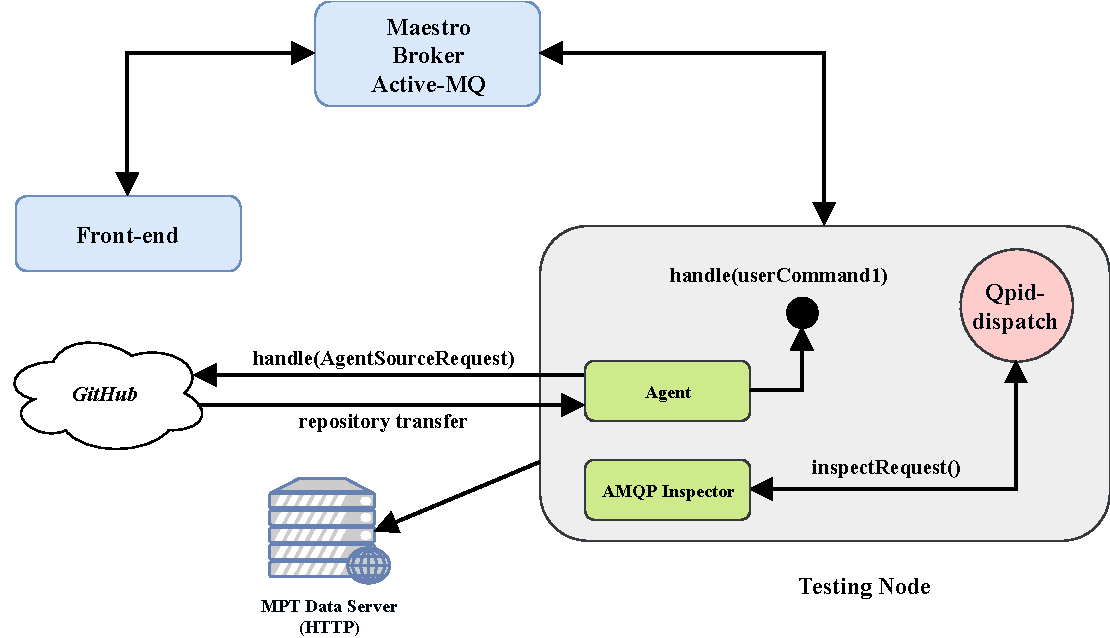
\includegraphics[width=13cm]{obrazky-figures/agent_demo.pdf}
  \caption{Communication inside the Maestro with agent notes handling depiction.}
  \label{fig:agent_demo}
\end{figure}

\todo{dopsat neco?}

\subsection{AMQP Management Inspector}
\label{AMQP Management Inspector}
The imformation collection about the router itself are not gathered by the agent. For this purpose, we developed new type of Maestro Inspector especially for AMQP Management. AMQP Management is layered on top of the AMQP protocol and it access the inner data about router by simple requests and responses. \todo{dopsat}

\subsection{Deployment Changes}
